\renewcommand{\FileName}{heplot-ideas}
\begin{frame}
  \frametitle{HE plots: Visualizing \mat{H} and \mat{E} (co) variation}

\begin{center}
  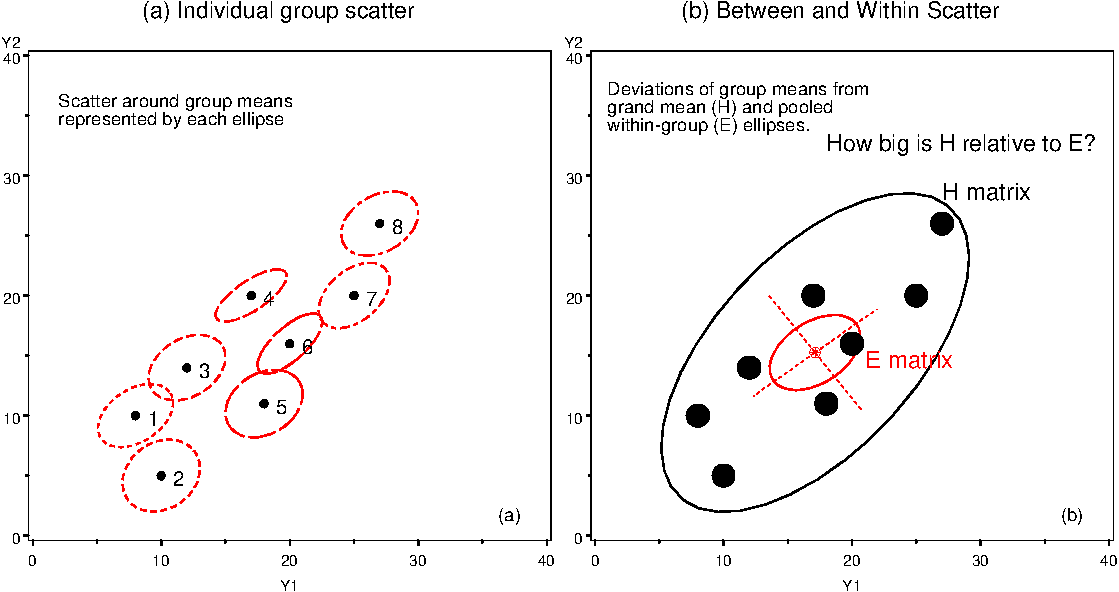
\includegraphics[width=.85\textwidth,clip]{fig/arcmanov1}
  \\ \black{Ideas behind multivariate tests: (a) Data ellipses; (b) \H and \E matrices}
\end{center}

\begin{itemize*}
  \item \mat{H} ellipse:  data ellipse for fitted values, $\hat{\vec{y}}_{ij} =
  \bar{\vec{y}}_j$.
  \item \mat{E} ellipse:  data ellipse of residuals, $\hat{\vec{y}}_{ij} -
  \bar{\vec{y}}_j$.
\end{itemize*}
\end{frame}

\begin{frame}
  \frametitle{HE plots: Visualizing multivariate hypothesis tests}
  \begin{center}
	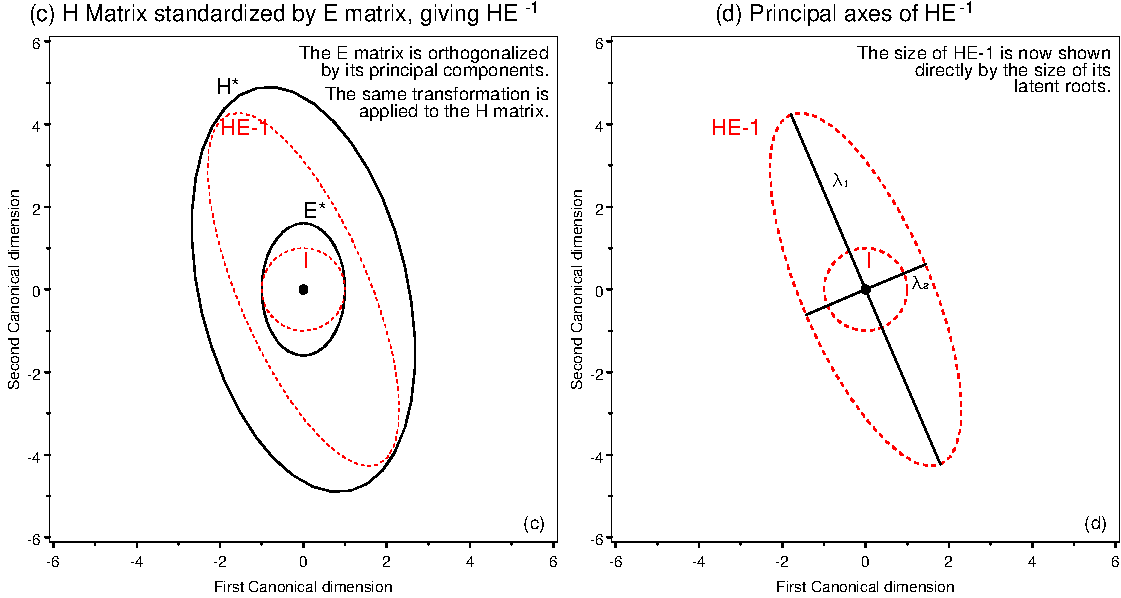
\includegraphics[width=.85\textwidth,clip]{fig/arcmanov2}
	\\ \black{Ideas behind multivariate tests: latent roots \& vectors of $\mat{H} \mat{E}^{-1}$}
  \end{center}
\begin{itemize*}
  \item $\lambda_i, i=1, \dots df_h$ show size(s) of \mat{H} relative to \mat{E}.
  \item latent vectors show canonical directions of maximal difference.
\end{itemize*}
\end{frame}

\begin{frame}
	\frametitle{HE plot for iris data}

  \begin{center}
	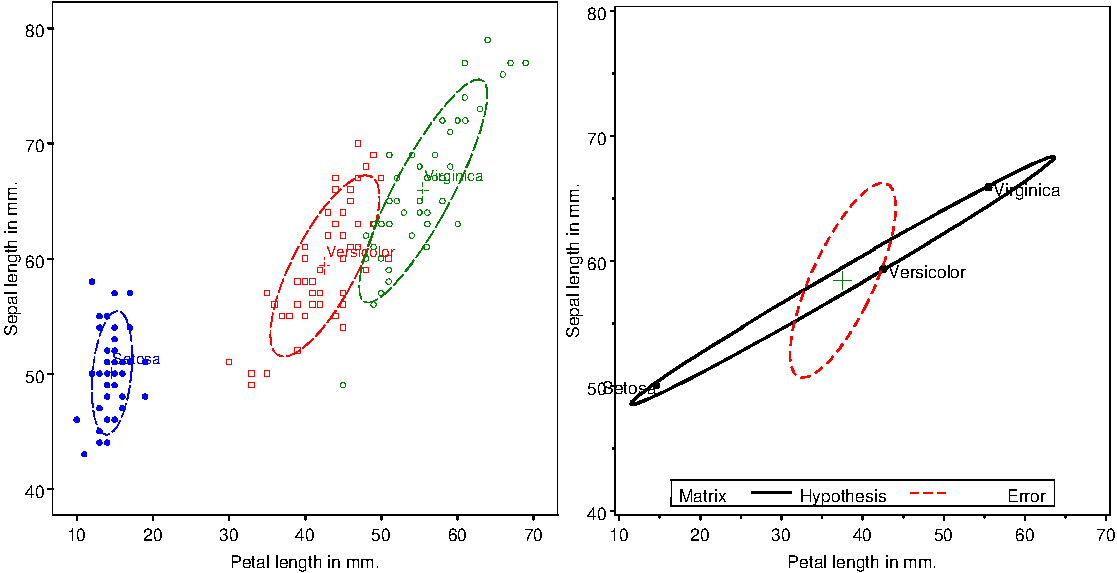
\includegraphics[width=.9\textwidth,clip]{fig/heplot31}
	\\ \black{(a) Data ellipses and (b) \H and \E matrices (scaled by $1/df_e$: effect size)}
  \end{center}
  \begin{itemize*}
  	\item \mat{H} ellipse:  data ellipse for fitted values, $\hat{\vec{y}}_{ij} =
	\bar{\vec{y}}_j$.
	\item \mat{E} ellipse:  data ellipse of residuals, $\hat{\vec{y}}_{ij} -
	\bar{\vec{y}}_j$.
  \end{itemize*}
\end{frame}


